\documentclass{beamer}

\usepackage[utf8]{inputenc}
\usepackage[T1]{fontenc}
\usepackage[english, italian]{babel}
\usepackage{tikz}

\setcounter{tocdepth}{1}

\definecolor{azzurro}{HTML}{E6E6FF}

\usetheme[compress]{Berlin}
\beamertemplatenavigationsymbolsempty

\title{Sviluppo di un'applicazione mobile cross-platform tramite l'uso di Appcelerator Titanium}
\author{Riccardo Bucco}
\institute[Università degli Studi di Padova]
{
	Dipartimento di Matematica\\
	Corso di Laurea in Informatica
}
\date{Padova, 17 febbraio 2016}


\begin{document}
	\begin{frame}[noframenumbering, plain]
		\titlepage
	\end{frame}

	\begin{frame}[noframenumbering]{Indice dei contenuti}
		\tableofcontents
	\end{frame}

	\addtobeamertemplate{navigation symbols}{}{%
		\usebeamerfont{footline}%
		\usebeamercolor[fg]{footline}%
		\hspace{1em}%
		\insertframenumber/\inserttotalframenumber
	}

	\chapter{Analisi del contesto aziendale}
	\section{L'azienda e il suo ambito di attività}
		PastBook è una piccola azienda con sede ad Amsterdam, nei Paesi Bassi. Essa offre agli utenti la possibilità di creare e stampare
		degli album fotografici personalizzati.
		\begin{figure}[H]
			\centering
			
\includegraphics[width=0.4\textwidth]{capitolo_1/immagini/logo_pastbook.png}
			\caption[Logo di PastBook]{Logo di PastBook\protect\footnotemark}
		\end{figure}
		\footnotetext{\url{https://fronteers.nl/_img/werkgevers/pastbook.png}}
		Il progetto nasce nel 2012 quando Stefano Cutello — fondatore e attuale titolare di PastBook — decide di abbandonare il posto di
		lavoro presso eBay per realizzare la propria idea. L'esigenza è quella di riscoprire i ricordi pubblicati ogni giorno sui social
		network: infatti, le vite delle persone sono ormai completamente online e non esiste più niente di stampato.\\
		L'azienda descrive il servizio che essa offre nel seguente modo:
		\hyphenblockquote{english}{Many things can disappear — not your memories. We believe that certain moments can last forever. We
			believe that the best things in the world are not things. We help you rediscover your memories. We collect the highlights of
			your life moments and provide you with a tangible way to relive them — in PastBook.}
		PastBook, dunque, aiuta le persone a raccogliere le proprie foto sparse per il Web e permette loro di creare un album fotografico
		che memorizzi in modo permanente i ricordi più belli.
	\section{Prodotti offerti}
		\subsection{Photo Books in un click}
			Esistono varie aziende che permettono agli utenti di creare album fotografici a partire dalle immagini presenti nei social
			network. PastBook differisce da esse per un importante principio che sta alla base della realizzazione del prodotto: l'utente
			deve poter creare il proprio Photo Book in modo veloce ed automatico, senza pensare a particolari che distolgano la sua mente
			dallo scopo.\\
			L'azienda prevede che i propri clienti debbano solo scegliere il servizio dal quale intendono ottenere le immagini. Il resto
			è automatico: non è previsto che l'utente abbia la possibilità di personalizzare il proprio Photo Book durante la sua
			realizzazione. I più esigenti possono fare piccole modifiche solo a creazione avvenuta.\\
			\begin{multicols}{3}[\noindent PastBook permette di recuperare le immagini utilizzando uno dei seguenti servizi Web:]
				\begin{itemize}
					\item Instagram
					\item Facebook
					\item Flickr
					\item Google Drive
					\item Dropbox
					\item OneDrive
					\item Picasa
					\item Evernote
					\item Box
				\end{itemize}
			\end{multicols}
			\begin{figure}
				\centering
				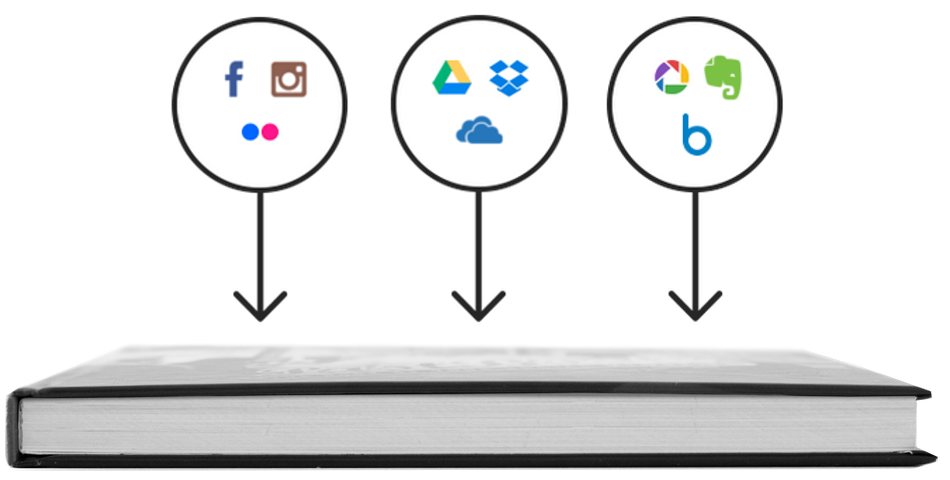
\includegraphics[width=0.9\textwidth]{capitolo_1/immagini/photo_book_one_click.png}
				\caption[Photo Book in un click]{Photo Book in un click\protect\footnotemark}
			\end{figure}
			\footnotetext{Immagine tratta da \url{https://www.pastbook.com/beautiful-photo-books/}}
			Gli utenti hanno inoltre la possibilità di invitare chiunque ad aggiungere ulteriori ricordi al proprio Photo Book,
			condividendo un link privato tramite email, QR code, Facebook o Twitter.
		\subsection{Photo Books personalizzati}
			PastBook offre anche una seconda tipologia di prodotti: Photo Book creati su misura da designer professionisti. Tale offerta
			è rivolta ai clienti che non pretendono risultati immediati ma che allo stesso tempo esigono una qualità superiore.
			\begin{figure}[H]
				\centering
				
\includegraphics[width=0.9\textwidth]{capitolo_1/immagini/photo_book_personalizzato.png}
				\caption[Realizzazione di un Photo Book personalizzato]{Realizzazione di un Photo Book personalizzato\protect\footnotemark}
			\end{figure}
			\footnotetext{Immagine tratta da \url{https://www.pastbook.com/elite/}}
			Gli utenti, in particolare, dopo aver mandato le proprie foto, possono interagire direttamente con la persona che si sta
			occupando della creazionde del Photo Book per indicare le immagini preferite o per esprimere eventuali preferenze
			riguardanti lo stile, i testi, i colori, etc.
	\section{Organizzazione aziendale}
		\subsection{Obiettivi e risultati attesi}
			PastBook persegue obiettivi di tre tipologie differenti:
			\begin{itemize}
				\item tecnici, legati al funzionamento dei prodotti;
				\item economici, legati alla produttività, all'efficacia e all'efficienza;
				\item sociali, legati alla qualità della vita e in particolare alla qualità della vita di lavoro.
			\end{itemize}
			\subsubsection{Qualità del prodotto e dei processi}
				Il principale obiettivo di PastBook è quello di realizzare un algoritmo che sia in grado di produrre in modo
				automatico un Photo Book che sia conforme alle aspettative dei clienti. Oltre a ciò, l'azienda intende raggiungere
				precisi traguardi riguardanti l'efficienza del processo di creazione del prodotto: esso deve avvenire nel minor tempo
				possibile e impiegando una quantità minima di risorse.\\
				Questi obiettivi puramente tecnici celano lo scopo economico di riuscire a vendere i Photo Book realizzati in modo
				automatico ad un prezzo inferiore rispetto a quello proposto della concorrenza, pur mantenendo elevata la
				soddisfazione dei clienti.
			\subsubsection{Semplicità di utilizzo degli strumenti}
				PastBook supporta da sempre una precisa filosofia: gli strumenti a disposizione degli utenti devono essere semplici,
				per non dire basilari. In particolare, l'azienda vuole che il cliente riesca ad ottenere qualcosa di gradito — non
				per forza perfetto — senza sentire il bisogno di dover intervenire per apportare modifiche.\\
				L'uso di questo tipo di approccio si basa sulle seguenti considerazioni:
				\begin{itemize}
					\item Spesso gli utenti provano un nuovo servizio per pura curiosità e, di conseguenza, non sono disposti ad
					utilizzare molto del proprio tempo per giungere al risultato. Numerose possibilità di modifiche e
					personalizzazioni non farebbero altro che spazientire l'utente. Un'azienda deve dunque saper sfruttare il
					breve contatto con il potenziale cliente per poterlo conquistare
					\item Quanto più è il tempo a disposizione di un utente per valutare un acquisto in modo razionale tanto
					meno influiscono su di esso impulsi ed emozioni. È dunque necessario saper cogliere l'irrazionalità iniziale
					del cliente per persuaderlo: per ottenere ciò, la quantità di azioni svolta per creare un Photo Book deve
					essere minima.
				\end{itemize}
			\subsubsection{Valorizzazione del capitale umano}
				Il titolare di PastBook è fermamente convinto che una forte cultura organizzativa sia un fattore critico per le
				performance e il successo dell'azienda. Egli, in particolare, cerca continuamente di motivare e coinvolgere i propri
				dipendenti per fare in modo che essi apprezzino i risultati che il loro lavoro può portare.\\
				In aggiunta, PastBook crede fortemente al fatto che la produttività del personale sia influenzata dalla qualità dei
				rapporti che si instaurano tra le persone facenti parte del team: ciascuno, con le proprie motivazioni, influenza
				positivamente gli altri individui del gruppo, facilitando il raggiungimento dei risultati imposti.\\
				\begin{figure}[H]
	\centering
	\begin{tikzpicture}
		\draw[fill=blue,fill opacity=0.1] (0,0) rectangle ++(0.19\textwidth,0.12\textwidth);
		\draw (0,0) rectangle ++(0.19\textwidth,0.12\textwidth)
		node[pos=.5, text width=0.18\textwidth, align=center] {Team di dipendenti};
		\draw[->] (0.20\textwidth,0.06\textwidth) -- (0.26\textwidth,0.06\textwidth);
		\draw[fill=blue,fill opacity=0.1] (0.27\textwidth,0) rectangle ++(0.19\textwidth,0.12\textwidth);
		\draw (0.27\textwidth,0) rectangle ++(0.19\textwidth,0.12\textwidth)
		node[pos=.5, text width=0.18\textwidth, align=center] {Spirito di squadra};
		\draw[->] (0.47\textwidth,0.06\textwidth) -- (0.53\textwidth,0.06\textwidth);
		\draw[fill=blue,fill opacity=0.1] (0.54\textwidth,0) rectangle ++(0.19\textwidth,0.12\textwidth);
		\draw (0.54\textwidth,0) rectangle ++(0.19\textwidth,0.12\textwidth)
		node[pos=.5, text width=0.18\textwidth, align=center] {Influenzamento reciproco};
		\draw[->] (0.74\textwidth,0.06\textwidth) -- (0.80\textwidth,0.06\textwidth);
		\draw[fill=blue,fill opacity=0.1] (0.81\textwidth,0) rectangle ++(0.19\textwidth,0.12\textwidth);
		\draw (0.54\textwidth,0) (0.81\textwidth,0) rectangle ++(0.19\textwidth,0.12\textwidth)
		node[pos=.5, text width=0.18\textwidth, align=center] {Obiettivi di produttività};
	\end{tikzpicture}
\end{figure}

				Infine, per fare in modo che ognuno esprima al meglio le proprie potenzialità, l'azienda intende decentralizzare le
				responsabilità ed aumentare l'autonomia decisionale. Parallelamente, ogni dipendente deve cercare di comprendere
				pienamente i limiti entro i quali può operare in modo autonomo.
		\subsection{Risorse disponibili}
			PastBook può avvalersi di numerose risorse per poter raggiungere gli obiettivi prefissati.\\
			Innanzitutto, l'azienda ha a disposizione i propri dipendenti e collaboratori: mentre alcuni di essi forniscono il proprio
			contributo solo per breve tempo, altri lavorano per PastBook in modo stabile. In particolare, durante il periodo in cui ho
			svolto lo stage, l'azienda era composta da 7-9 persone. In aggiunta, alcuni mentori che hanno contribuito a far crescere
			PastBook durante i suoi esordi offrono spesso il proprio aiuto per individuare le strategie vincenti.\\
			Per quanto riguarda le risorse economiche, l'azienda può fare affidamento su una serie di investitori privati che credono
			fortemente nel progetto e nelle persone che lo stanno realizzando. Essi forniscono perlopiù sostegno finanziario e non hanno
			ruoli di tipo decisionale.\\
			Le risorse tecnologiche necessarie all'azienda sono molto poche. Infatti, ogni persona lavora utilizzando il proprio PC e
			solo in casi particolari utilizza dispositivi di altro tipo.\\
			Per quanto riguarda gli spazi, infine, i dipendenti di PastBook possono usufruire, oltre che dell'ufficio, anche di due
			cucine e di una sala relax.
		\subsection{Componenti e relazioni organizzative}
			\subsubsection{Funzioni e ruoli}
				In PastBook le responsabilità di ciascuna persona sono ben definite. Questo aiuta i dipendenti a capire i propri
				confini operativi e a diminuire le dimenticanze.\\
				L'azienda — per funzionare in modo corretto — necessita dei seguenti ruoli:
				\begin{center}
					\rowcolors{1}{azzurro_chiaro}{azzurro}
					\begin{tabular}[H]{p{0.25\textwidth} p{0.60\textwidth}}
						Dirigente 			& Si occupa della gestione delle risorse disponibili e del
										  coordinamento generale per poter raggiungere gli obiettivi
										  prefissati.\\
						\hline
						Responsabile finanziario	& Si occupa della gestione e della supervisione delle attività
										  finanziarie.\\
						\hline
						Responsabile del marketing	& Si occupa della comunicazione sui social media, attuando strategie
										  per aumentare il valore percepito dai consumatori rispetto al
										  prodotto offerto.\\
					\end{tabular}
				\end{center}
				\begin{center}
					\rowcolors{1}{azzurro}{azzurro_chiaro}
					\begin{tabular}[H]{p{0.25\textwidth} p{0.60\textwidth}}
						Customer relationship manager	& Si occupa della gestione delle relazioni con i clienti. Questo
										  implica un approccio operativo (risposte tempestive ed efficaci
										  alle richieste) e uno analitico (analisi dei bisogni e della
										  soddisfazione per sviluppare un'offerta commerciale appropriata).\\
						Grafico				& Fornisce supporto e consulenza artistica durante la progettazione
										  dei vari prodotti (sito web, applicazioni mobile, banner
										  pubblicitari, etc.).\\
						\hline
						Chief technical officer		& Supervisiona l'implementazione dei prodotti e dei servizi offerti
										  per assicurare che portino valore aggiunto all'azienda. Coglie le
										  potenzialità di nuove tecnologie per convertirle in decisioni
										  strategiche per l'azienda.\\
						\hline
						Sviluppatore 			& Si occupa dei vari aspetti del ciclo di vita di un prodotto
										  software.\\
					\end{tabular}
				\end{center}
				Alcuni dipendenti aziendali, a seconda delle necessità, possono ricoprire più di una mansione.
			\subsubsection{Struttura organizzativa}
				L'azienda è suddivisa in tre unità organizzative, individuate sulla base degli obiettivi che ognuna di esse si impone
				di raggiungere:
				\begin{itemize}
					\item all'\emph{area amministrativa}, che si occupa di aspetti economici e decisionali, appartengono il
					dirigente e il responsabile finanziario;
					\item all'\emph{area commerciale}, che si occupa delle strategie di mercato, della commercializzazione del
					prodotto e dell'assistenza ai clienti, appartengono tutti i membri del front office e il responsabile del
					marketing;
					\item all'\emph{area ricerca e sviluppo}, che studia come migliorare i prodotti o come crearne di nuovi,
					appartengono il CTO, gli sviluppatori e il grafico.
				\end{itemize}
				\begin{figure}[H]
	\centering
	\begin{tikzpicture}
		\draw[fill=azzurro] (0,0) rectangle ++(0.20\textwidth,0.12\textwidth);
		\draw (0,0) rectangle ++(0.20\textwidth,0.12\textwidth)
		node[pos=.5, text width=0.18\textwidth, align=center] {Area commerciale};
		\draw[fill=azzurro] (0.56\textwidth,0) rectangle ++(0.20\textwidth,0.12\textwidth);
		\draw (0.56\textwidth,0) rectangle ++(0.20\textwidth,0.12\textwidth)
		node[pos=.5, text width=0.18\textwidth, align=center] {Area ricerca e sviluppo};
		\draw[fill=azzurro] (0.28\textwidth,0.13\textwidth) rectangle ++(0.20\textwidth,0.12\textwidth);
		\draw (0.28\textwidth,0.13\textwidth) rectangle ++(0.20\textwidth,0.12\textwidth)
		node[pos=.5, text width=0.18\textwidth, align=center] {Area amministrativa};
		\draw (0.21\textwidth,0.06\textwidth) -- (0.55\textwidth,0.06\textwidth);
		\draw (0.38\textwidth,0.06\textwidth) -- (0.38\textwidth,0.12\textwidth);
	\end{tikzpicture}
\end{figure}

				PastBook, essendo una realtà aziendale molto piccola, non prevede la presenza di organi di comando e relativi
				subordinati. Tuttavia, per ognuna delle unità organizzative è possibile individuare una persona che funge da
				riferimento per i colleghi: una sorta di leader informale, che trae la sua legittimazione dal consenso degli altri
				membri.\\
				Molto spesso — per far fronte a nuovi problemi o per tentare di raggiungere specifici obiettivi — persone provenienti
				da unità diverse formano dei gruppi di lavoro temporanei, non descrivibili all'interno dell'organigramma. Questi
				gruppi sono formati per sfruttare competenze in ambiti diversi e per affrontare i problemi da diversi punti di vista.
				Accade spesso, per esempio, che gli esperti di marketing collaborino con i membri dell'area ricerca e sviluppo per
				poter realizzare un prodotto di valore sia dal punto di vista funzionale che commerciale.
			\subsubsection{Coordinamento e controllo}
				Stefano Cutello — attuale dirigente di PastBook — ha un duplice compito: gestire le attività correnti dell'azienda e
				contemporaneamente cercare nuove opportunità, prevedendo i mutamenti e sviluppando una strategia interna attraverso
				la conoscenza del contesto esterno. Oltre che manager, egli è anche il leader effettivo del team: ha la capacità di
				comunciare, di interagire, di gestire le relazioni. In particolare, egli motiva costantemente i suoi collaboratori a
				dare il meglio di sé per poter raggiungere gli obiettivi prefissati.\\
				Per controllare e coordinare il flusso delle attività in azienda, Stefano ha scelto di applicare una tecnica molto
				simile allo Scrum. Ogni mattina, prima di cominciare a lavorare, avviene il cosiddetto \emph{daily standup}, un
				breve incontro durante il quale ogni membro del team prende la parola per pochi minuti e spiega agli altri due cose:
				\begin{itemize}
					\item che attività ha svolto il giorno precedente precedente e quali risultati ha ottenuto (gli obiettivi
					fissati sono stati raggiunti?);
					\item cosa intende fare il giorno stesso e quali risultati vuole ottenere (quali obiettivi si pone?).
				\end{itemize}
				Durante il meeting giornaliero ognuno è anche invitato a condividere dubbi, ostacoli o impedimenti emersi durante le
				proprie attività: in questo modo è possibile ricevere consigli o aiuto diretto da parte dei colleghi.\\
				Per controllare il lavoro di ciascuno, inoltre, il dirigente utilizza
				\emph{Trello}\footnote{Applicazione web che permette di rappresentare un progetto tramite una \emph{board} che contiene alcune \emph{lists} (corrispondenti a liste
di task). Ogni list contiene delle \emph{cards} (corrispondenti a task). Le card possono essere spostate da una lista alla successiva, tramite un
semplice \emph{drag-and-drop}.}
. Nello specifico, ogni dipendente ha accesso alle board riguardanti
				i progetti ai quali collabora. Ogni board è composta da tre liste: \emph{TODO} (contenente ciò che non è ancora
				stato fatto), \emph{DOING} (che contiene informazioni riguardanti quanto è in corso d'opera) e \emph{DONE} (un
				elenco dei task portati a termine). Ogni membro di una certo progetto deve preoccuparsi di mantenere aggiornate le
				posizioni delle card a lui assegnate all'interno della board. In questo modo il dirigente o il responsabile di un
				progetto è sempre in grado di capire quanto manchi al raggiungimento degli obiettivi prefissati.\\
				Per permettere un coordinamento più generale, oltre ai brevi incontri giornalieri in azienda sono previste riunioni
				con cadenza mensile alle quali tutti i membri del team sono invitati a partecipare tramite il proprio contributo.
				Questi meeting sono più impegnativi rispetto ai daily standup (durano fino a quattro ore) e includono i seguenti
				elementi:
				\begin{itemize}
					\item Ogni unità organizzativa riassume quanto è avvenuto durante il mese trascorso, con particolare
					riferimento all'eventuale raggiungimento degli obiettivi fissati. In particolare, l'area amministrativa
					riporta i dati riguardanti la situazione finanziaria, l'area commerciale si concentra sull'uso che la
					clientela fa dei servizi e sul funzionamento delle campagne pubblicitarie, l'area ricerca e sviluppo mostra
					i progressi fatti nella realizzazione di nuovi prodotti.
					\item Ogni membro del team esamina e commenta i dati riportati dalle varie unità, identificando cosa è andato
					bene e cosa possa essere potenzialmente migliorato. Al termine di questa attività il team fissa obiettivi
					concreti da raggiungere nel mese seguente.
					\item Il dirigente pianifica il lavoro che deve essere svolto per poter raggiungere gli obiettivi fissati e
					delega le varie responsabilità. Eventualmente egli dispone che alcuni dipendenti formino dei gruppi di
					progetto per poter affrontare e risolvere dati problemi.
				\end{itemize}
			\subsubsection{Gestione del personale}
				Il personale è una dei fattori di successo di PastBook: i dipendenti sono molto coinvolti nei processi decisionali
				ed è richiesta loro una grande flessibilità nel ricoprire mansioni all'interno dell'azienda. Di conseuenza, il ruolo
				di chi si occupa del personale è fondamentale.\\
				La gestione delle risorse umane svolge prevalentemente le seguenti attività:
				\begin{itemize}
					\item selezionare e formare;
					\item motivare e coinvolgere.
				\end{itemize}
				Innanzitutto, l'efficienza e la potenzialità di PastBook dipendono in larga misura dall'attenta \emph{selezione} dei
				collaboratori: eventuali errori commessi in tale fase comportano conseguenze negative per l'azienda. Il processo
				selettivo comporta un'attenta analisi delle capacità, abilità e caratteristiche personali degli individui esaminati.
				In particolare, per l'azienda è importante che essi siano in larga misura indipendenti nel modo di lavorare e nel
				saper prendere decisioni ponderate e sensate nei momenti di difficoltà.\\
				In secondo luogo, l'azienda riconosce l'importanza della \emph{formazione} del personale: gli individui che sono
				stati inseriti nel team necessitano di un rapido potenziamento delle conoscenze e delle capacità per poter lavorare
				in autonomia quanto prima. L'obiettivo del processo formativo è raggiunto grazie all'attuazione di percorsi di
				affiancamento: essi permettono al nuovo membro del gruppo di capire sia il metodo di lavoro utilizzato a PastBook che
				le regole e i valori che non sono stati formalizzati.\\
				L'ultimo compito di coloro che gestiscono le risorse umane è quello di \emph{motivare} e allo stesso tempo
				\emph{coinvolgere} il personale, facendo in modo che i dipendenti abbiano un atteggiamento mentale positivo nei
				confronti dei loro compiti e responsabilità. Per poter raggiungere questi obiettivi, il team è costantemente
				stimolato a cimentarsi in nuove esperienze e a proporre nuove idee. Inoltre, i legami di amicizia fra colleghi sono
				incoraggiati tramite attività terze da svolgere eventualmente anche durante l'orario di lavoro.
			\subsubsection{Gestione dei clienti}
				PastBook cerca costantemente di sviluppare un orientamento strategico che pone l'attenzione sulla costruzione e il
				mantenimento di una base di clienti fedeli che siano in grado di incrementare la redditività nel medio-lungo
				termine.\\
				L'enfasi posta sullo sviluppo nel tempo di relazioni con la clientela — piuttosto che soltanto sulla chiusura di una
				singola transazione di vendita — comporta numerosi vantaggi. Innanzitutto, i ricavi incrementano grazie a una
				riduzione dei costi, dovuta soprattutto a un mercato nel quale si gioca a sottrarre clienti alla concorrenza tramite
				azioni promozionali aggressive rivolte ai nuovi utenti. In secondo luogo, l'azienda può contare su un flusso costante
				di entrate. Inoltre, clienti fedeli (e dunque soddisfatti) danno spesso origine a un passaparola che, se assume una
				consistenza significativa, può contribuire notevolmente al miglioramento dell'immagine aziendale. Infine, un
				vantaggio di natura immateriale riguarda la possibilità di sviluppare più facilmente soluzioni innovative: i clienti,
				se correttamente coinvolti nel processo di miglioramento del prodotto, possono proporre idee che incrementino la
				competitività stessa dell'azienda.
				\begin{figure}[H]
	\centering
	\begin{tikzpicture}
		\draw[fill=azzurro] (0,0) rectangle ++(0.22\textwidth,0.12\textwidth);
		\draw (0,0) rectangle ++(0.22\textwidth,0.12\textwidth)
		node[pos=.5, text width=0.17\textwidth, align=center] {Minori costi di gestione};
		\draw[fill=azzurro] (0.26\textwidth,0) rectangle ++(0.22\textwidth,0.12\textwidth);
		\draw (0.26\textwidth,0) rectangle ++(0.22\textwidth,0.12\textwidth)
		node[pos=.5, text width=0.17\textwidth, align=center] {Flussi di entrate costanti};
		\draw[fill=azzurro] (0.52\textwidth,0) rectangle ++(0.22\textwidth,0.12\textwidth);
		\draw (0.52\textwidth,0) rectangle ++(0.22\textwidth,0.12\textwidth)
		node[pos=.5, text width=0.17\textwidth, align=center] {Passaparola positivo};
		\draw[fill=azzurro] (0.78\textwidth,0) rectangle ++(0.22\textwidth,0.12\textwidth);
		\draw (0.78\textwidth,0) rectangle ++(0.22\textwidth,0.12\textwidth)
		node[pos=.5, text width=0.17\textwidth, align=center] {Collaborazione con i clienti orientati all'innovazione};
		\draw (0.11\textwidth,0.19\textwidth) -- (0.89\textwidth,0.19\textwidth);
		\draw[->] (0.11\textwidth,0.19\textwidth) -- (0.11\textwidth,0.13\textwidth);
		\draw[->] (0.37\textwidth,0.19\textwidth) -- (0.37\textwidth,0.13\textwidth);
		\draw[->] (0.63\textwidth,0.19\textwidth) -- (0.63\textwidth,0.13\textwidth);
		\draw[->] (0.89\textwidth,0.19\textwidth) -- (0.89\textwidth,0.13\textwidth);
		\draw (0.50\textwidth,0.19\textwidth) -- (0.50\textwidth,0.25\textwidth);
		\draw[fill=azzurro_scuro] (0.39\textwidth,0.26\textwidth) rectangle ++(0.22\textwidth,0.12\textwidth);
		\draw (0.39\textwidth,0.26\textwidth) rectangle ++(0.22\textwidth,0.12\textwidth)
		node[pos=.5, text width=0.17\textwidth, align=center] {Cliente fedele};
	\end{tikzpicture}
\end{figure}

				Per aumentare la fedeltà e il grado di soddisfazione della clientela, l'area aziendale dedicata alle relazioni con
				i clienti svolge due attività:
				\begin{itemize}
					\item \emph{Assistenza personalizzata}, ovvero aiuto rivolto agli utenti che riscontrano problemi durante
					l'utilizzo dei prodotti offerti da PastBook. L'operatore aziendale, oltre a fornire le corrette	indicazioni
					richieste, si preoccupa di raccogliere dati che riguardano come il prodotto è percepito dal cliente. Questi
					dati sono poi rielaborati dall'amministrazione per cercare di pianificare e attuare strategie commerciali
					adatte.
					\item {Mantenimento di un blog} aziendale nel quale sono inseriti sia suggerimenti su come usare gli
					strumenti messi a disposizione da PastBook che fatti, eventi e curiosità che possono stuzzicare la mente del
					lettore. Il blog è innanzitutto lo strumento grazie al quale l'azienda suggerisce implicitamente delle
					occasioni durante le quali un cliente può pensare di realizzare e comprare un Photo Book. In secondo luogo il
					blog è il mezzo tramite cui il pubblico è informato delle novità introdotte e delle promozioni in corso.
				\end{itemize}
			\subsubsection{Comunicazione nell'azienda}
				I dipendenti aziendali comunicano tra loro prevalentemente tramite contatti informali, fortemente basati sulle
				relazioni. Non è presente alcun tipo di struttura gerarchica che preveda controlli sui modi di comunicare tra membri
				appartenenti ad aree differenti dell'azienda. Questo modo di comunicare è fortemente dovuto al fatto che tutto il
				personale lavori all'interno di una stessa grande stanza.\\
				Il principale strumento informatico di supporto alla comunicazione è \emph{Slack}\footnote{\url{http://www.slack.com} Strumento di collaborazione multipiattaforma, ideale per i team di lavoro. Questo tool annovera le funzionalità
ormai “classiche” delle chat, tra le quali la possibilità di creare canali di comunicazione tematici, di riservare messaggi a determinati colleghi e
di condividere file. Inoltre, esso garantisce numerosi altri vantaggi a coloro che lo usano per lavorare in gruppo: collaborazione durante la modifica
di \emph{snippet} di codice, \emph{screen sharing} e comunicazione video. Il vero punto di forza, tuttavia, è rappresentato dalla possibilità di
integrazione con centinaia dei più importanti software presenti sul mercato (Twitter, Dropbox, GitHub, Heroku, Trello etc.).}
:
				ogni unità organizzativa aziendale e ogni gruppo di progetto possiede un proprio canale nel quale possono essere
				ospitate conversazioni, scambiati file e condivise porzioni di codice.
	\section{Sviluppo software}
		\subsection{Metodologia di lavoro}
			\subsubsection{Tipico ciclo di vita del software}
				L'idea alla base di un prodotto software sviluppato da PastBook deriva molto spesso dal contributo portato
				dall'intero team durante i meeting mensili. Queste occasioni, infatti, danno l'opportunità ai dipendenti di esprimere
				la propra opinione con lo scopo di migliorare la qualità dei servizi e dei prodotti offerti dall'azienda. Quando il
				concetto proposto dimostra di poter essere di effettivo valore, il dirigente sceglie alcuni membri del team e li
				assegna a un gruppo di progetto dedicato.\\
				Il passo successivo nello sviluppo dell'idea consiste solitamente in una breve analisi dei requisiti, durante la
				quale il gruppo cerca di delineare le caratteristiche e i requisiti che il prodotto dovrà avere. Ogni membro del
				gruppo individua contemporaneamente quale sia la propria parte di lavoro e come questa possa successivamente
				integrarsi con le attività svolte dai colleghi.\\
				A questo punto, a seconda delle abilità e delle capacità presenti nel gruppo di lavoro, lo sviluppo del prodotto
				si divide parti in distinte:
				\begin{itemize}
					\item Gli sviluppatori sono sempre presenti. Essi sono eventualmente coordinati dal CTO. Il loro compito è
					di progettare e codificare in modo appropriato le varie funzionalità individuate durante l'attività di
					analisi.
					\item Se il prodotto è destinato al pubblico allora quasi sempre il grafico comincia a delineare
					l'interfaccia. Egli sta in stretto contatto con gli sviluppatori, aggiornandoli su eventuali requisiti
					che essi devono soddisfare.
					\item Molto spesso nella realizzazione del prodotto sono coinvolti dipendenti che hanno capacità commerciali.
					Essi svolgono prevalentemente funzioni di supporto a chi si occupa della grafica. Infatti, danno indicazioni
					sui metodi migliori per interagire con la clientela e per intrattenerla e coinvolgerla allo stesso tempo.
				\end{itemize}
				Obiettivo primario di qualsiasi gruppo di progetto software all'interno di PastBook è sempre quello di mettere a
				disposizione del resto del'azienda un prototipo funzionante nel minor tempo possibile: in questo modo il prodotto può
				essere testato dall'intero team. Infine, quando il prototipo raggiunge una maturità sufficiente, esso è distribuito
				anche ad utenti esterni a PastBook, in modo tale che ne possano testare le funzionalità.\\
				Dopo il rilascio del prodotto, il gruppo di progetto si scioglie. Quando insorgono problemi e si rende necessaria
				attività di manutenzione, il dirigente delega la responsabilità a un dipendente adatto alla mansione.
				\begin{figure}[H]
	\centering
	\begin{tikzpicture}
		\draw[fill=azzurro] (0,0.60\textwidth) rectangle ++(0.24\textwidth,0.10\textwidth);
		\draw (0,0.60\textwidth) rectangle ++(0.24\textwidth,0.10\textwidth)
		node[pos=.5, text width=0.22\textwidth, align=center] {Concepimento idea e formazione dei gruppo di lavoro};
		
		\draw (0.25\textwidth,0.65\textwidth) -- (0.28\textwidth,0.65\textwidth);
		\draw[->] (0.28\textwidth,0.65\textwidth) -- (0.28\textwidth,0.59\textwidth);
		
		\draw[fill=azzurro] (0.16\textwidth,0.48\textwidth) rectangle ++(0.24\textwidth,0.10\textwidth);
		\draw (0.16\textwidth,0.48\textwidth) rectangle ++(0.24\textwidth,0.10\textwidth)
		node[pos=.5, text width=0.22\textwidth, align=center] {Analisi dei requisiti};
		
		\draw (0.41\textwidth,0.53\textwidth) -- (0.44\textwidth,0.53\textwidth);
		\draw[->] (0.44\textwidth,0.53\textwidth) -- (0.44\textwidth,0.47\textwidth);
		
		\draw (0.31\textwidth,0.12\textwidth) rectangle ++(0.26\textwidth,0.34\textwidth);
		
		\draw[fill=azzurro] (0.32\textwidth,0.35\textwidth) rectangle ++(0.24\textwidth,0.10\textwidth);
		\draw (0.32\textwidth,0.35\textwidth) rectangle ++(0.24\textwidth,0.10\textwidth)
		node[pos=.5, text width=0.22\textwidth, align=center] {Progettazione del software e codifica};
		
		\draw[fill=azzurro] (0.32\textwidth,0.24\textwidth) rectangle ++(0.24\textwidth,0.10\textwidth);
		\draw (0.32\textwidth,0.24\textwidth) rectangle ++(0.24\textwidth,0.10\textwidth)
		node[pos=.5, text width=0.22\textwidth, align=center] {Ideazione interfaccia grafica};
		
		\draw[fill=azzurro] (0.32\textwidth,0.13\textwidth) rectangle ++(0.24\textwidth,0.10\textwidth);
		\draw (0.32\textwidth,0.13\textwidth) rectangle ++(0.24\textwidth,0.10\textwidth)
		node[pos=.5, text width=0.22\textwidth, align=center] {Analisi del bisogno dei clienti};
		
		\draw (0.50\textwidth,0.47\textwidth) -- (0.50\textwidth,0.50\textwidth);
		\draw[->] (0.50\textwidth,0.50\textwidth) -- (0.69\textwidth,0.50\textwidth);
		
		\draw[dashed] (0.59\textwidth,0.50\textwidth) -- (0.55\textwidth,0.55\textwidth);
		\draw (0.47\textwidth,0.55\textwidth) rectangle ++(0.16\textwidth,0.08\textwidth)
		node[pos=.5, text width=0.16\textwidth, align=center] {Realizzazione prototipo};
		
		\draw (0.82\textwidth,0.44\textwidth) -- (0.82\textwidth,0.41\textwidth);
		\draw[->] (0.82\textwidth,0.41\textwidth) -- (0.58\textwidth,0.41\textwidth);
		
		\draw[dashed] (0.70\textwidth,0.41\textwidth) -- (0.75\textwidth,0.36\textwidth);
		\draw (0.67\textwidth,0.28\textwidth) rectangle ++(0.16\textwidth,0.08\textwidth)
		node[pos=.5, text width=0.16\textwidth, align=center] {Resoconti dei problemi};
		
		\draw[fill=azzurro] (0.70\textwidth,0.45\textwidth) rectangle ++(0.24\textwidth,0.10\textwidth);
		\draw (0.70\textwidth,0.45\textwidth) rectangle ++(0.24\textwidth,0.10\textwidth)
		node[pos=.5, text width=0.22\textwidth, align=center] {Collaudo};
		
		\draw (0.58\textwidth,0.29\textwidth) -- (0.61\textwidth,0.29\textwidth);
		\draw[->] (0.61\textwidth,0.29\textwidth) -- (0.61\textwidth,0.11\textwidth);
		
		\draw[fill=azzurro] (0.49\textwidth,0) rectangle ++(0.24\textwidth,0.10\textwidth);
		\draw (0.49\textwidth,0) rectangle ++(0.24\textwidth,0.10\textwidth)
		node[pos=.5, text width=0.22\textwidth, align=center] {Rilascio del prodotto};
	\end{tikzpicture}
	\caption{Ciclo di vita del software}
\end{figure}

			\subsubsection{Analisi dei requisiti}
				I gruppi di lavoro svolgono l'analisi dei requisiti durante le prime fasi di un progetto. In generale, il compito di
				tale attività è quello di chiarire e dettagliare le caratteristiche e le funzioni che deve possedere il prodotto
				finale.\\
				Le direttive aziendali non prevedono che i dipendenti che svolgono questi compiti dedichino parte del loro tempo alla
				produzione di una documentazione formale. Dunque, i dati raccolti durante attività quali la definizione del
				problema, l'analisi di fattibilità e l'analisi del dominio non sono in alcun modo memorizzati in modo persistente.
				Non esiste nemmeno una vero e proprio documento che contenga la specifica dei requisiti. Infatti, i membri del
				gruppo di lavoro si limitano a utilizzare appunti, diagrammi e disegni fatti a mano: un incaricato, in seguito, si
				occupa della loro digitalizzazione e memorizzazione, senza però seguire alcun tipo di norma esplicita.\\
				Questo modo di procedere informale e talvolta impreciso ha diverse conseguenze. Innanzitutto, i requisiti sono 
				talvolta soggetti a intepretazione. In secondo luogo, essi possono mutare spesso durante le fasi successive dello
				sviluppo del prodotto.
			\subsubsection{Progettazione e codifica}
				La progettazione — intesa come attività che entra nel merito della struttura del sistema software, definendo come i
				requisiti devono essere soddisfatti — è un'esclusiva degli sviluppatori e del CTO.\\
				Tale attività intermedia tra analisi dei requisiti e codifica trova pochissimo spazio all'interno del ciclo di vita
				del software: l'obiettivo principale dell'azienda è poter ottenere un prototipo che funzioni quanto prima e la
				progettazione è ritenuta un formalismo che fa perdere tempo prezioso. Di conseguenza, non esiste alcun tipo di
				documentazione formale o informale che descrivi l'architettura del sistema e come essa si scomponga in moduli.\\
				Gli sviluppatori, piuttosto, devono essere esperti al punto tale da avere fin dall'inizio un'idea abbastanza precisa
				della struttura finale del sistema. La codifica, dunque, rappresenta l'attività predominante durante l'intero
				processo di sviluppo, poiché include in modo implicito molti dei compiti che dovrebbero essere assegnati a dei
				progettisti.\\
				PastBook è a conoscenza del fatto che questo approccio è molto rischioso nel medio e lungo termine: cambiamenti
				nell'architettura di un sistema software durante uno stato avanzato della produzione possono implicare ingenti
				perdite di energie, tempo e denaro. Tuttavia, l'azienda non vuole rinunciare al vantaggio di poter ottenere fin dalle
				fasi iniziali un prototipo funzionante del prodotto. Dunque, per evitare che errori gravi rischino di bloccare la
				realizzazione del prodotto, il dirigente di PastBook invita spesso gli sviluppatori a svolgere sessioni di
				\emph{pair programming}: queste permettono un confronto diretto sul campo per poter individuare le maggiori
				criticità.\\
				Per concludere, i programmatori si preoccupano costantemente di mantenere il codice sorgente ben strutturato e
				commentato, essendo esso l'unica forma di documentazione dalla quale trarre informazioni riguardanti il sistema
				software in questione. Anche il controllo di versione e la descrizione delle modifiche apportate di volta in volta
				sono eseguiti con particolare cura.
			\subsubsection{Collaudo}
				Tale attività serve per individuare le carenze di correttezza, completezza e affidabilità delle componenti software
				in corso di sviluppo.\\
				L'azienda prevede che per ogni prodotto siano eseguiti degli \emph{alpha test}: in pratica, il personale di PastBook
				sottopone il software a collaudo prima di procedere alla distribuzione al pubblico. Questi test — anche se non sono
				solitamente formalizzati e preparati a priori — sono molto specifici e coprono una parte significativa dei possibili
				casi d'uso. I programmatori, inoltre, prima di sottoporre il software a questo tipo di collaudo, arricchiscono il
				codice con istruzioni di controllo a runtime che facilitino il rilevamento degli errori.\\
				Il gruppo di lavoro, infine, distribuisce a individui esterni all'azienda alcuni prototipi che risultino abbastanza
				stabili e che abbiano superato con successo i test interni. Tali utenti eseguono i cosiddetti \emph{beta test}. In
				questo modo PastBook raggiunge due obiettivi:
				\begin{itemize}
					\item Utenti selezionati possono provare in anteprima i prodotti aziendali. Queste persone sono normalmente
					giornalisti o blogger che desiderano svelare in anteprima le funzionalità di un nuovo prodotto. L'azienda ha
					così la possibilità di pubblicizzare il proprio marchio. Talvolta i prodotti sono consegnati anche a
					possibili investitori che possono valutare le potenzialità di PastBook.
					\item Gli utenti usano il software in casi realistici e inviano al produttore resoconti dei malfunzionamenti
					riscontrati. Il gruppo di lavoro raccoglie in modo minuzioso i dati provenienti dai beta test per poi
					utilizzarli nell'individuazione e correzione di eventuali errori.
				\end{itemize}
				Ovviamente, gli sviluppatori sfruttano gli utenti esterni solo per testare i prodotti che sono pensati per il
				pubblico. Il software necessario al funzionamento interno di PastBook non viene reso noto al di fuori dei confini
				dell'azienda.
		\subsection{Tecnologie, tecniche e strumenti utilizzati}
			\subsubsection{Generazione di un Photo Book}
				L'azienda ha trovato un modo semplice ed efficace di generare i Photo Book, utilizzando in gran parte una tecnologia
				stabile ed affermata: \emph{WebKit}\footnote{Motore di rendering per pagine web. Al giorno d'oggi, alcuni dei principali browser sul mercato (quali Google Chrome, Opera e Safari) si
basano su di esso.}
. In particolare, l'algoritmo sviluppato da
				PastBook non fa altro che utilizzare la funzione che converte una pagina composta da codice HTML e CSS in un
				documento PDF: la stessa che browser come Google Chrome utilizzano per dare all'utente la possibilità di esportare i
				contenuti web nel formato sviluppato da Adobe Systems.\\
				L'utilizzo automatizzato di tale tecnologia è possibile grazie ai cosiddetti
				\emph{headless browser}\footnote{Web browser senza interfaccia grafica, eseguibile da linea di comando.} 
. PastBook, per esempio, fa uso di Google Chrome
				e delle API del suo motore di rendering che sono messe a disposizione degli sviluppatori.\\
				Il problema risulta dunque semplificato: ciò che il software aziendale deve fare è creare dinamicamente una
				rappresentazione formale del documento, senza preoccuparsi del suo successivo rendering. In particolare, l'algoritmo
				definisce innanzitutto la struttura dell'album tramite l'uso del linguaggio HTML e utilizzando le foto messe a
				disposizione dall'utente. In secondo luogo, aggiunge un foglio di stile CSS per formattare il contenuto
				precedentemente creato. WebKit porta a termine il resto del lavoro, generando il documento PDF a partire dai dati
				prodotti dal software PastBook.\\
				L'algoritmo dell'azienda è complesso non tanto nel rendering dell'album quanto nella creazione di una struttura e di
				una formattazione appropriata. Infatti, esso si occupa di disporre le immagini fornite in un modo che risulti
				gradevole all'utente. Inoltre, esso tenta di capire quali sono le foto migliori — qualsiasi cosa questo voglia dire —
				e quale di queste può essere scelta come copertina del Photo Book. L'algoritmo, allo stesso tempo, deve essere molto
				veloce, poichè gli utenti pretendono risultati istantanei.
			\subsubsection{API e Service}
				L'infrastruttura dei server di PastBook si base su due concetti fondamentali: \emph{API} e \emph{Service}.\\
				Il primo di questi concetti risponde esattamente alla definizione di web API che fornisce la letteratura:
				un'interfaccia di programmazione per un server web che è accessibile attraverso un endpoint e che permette a chi la
				usa di espletare un determinato compito. In particolare, le API aziendali mettono a disposizione degli sviluppatori
				le funzionalità basilari di cui essi hanno bisogno. Alcuni esempi sono:
				\begin{itemize}
					\item autenticazione al server PastBook
					\item creazione di un Photo Book vuoto
					\item aggiunta di una foto ad un Photo Book
					\item sostituzione della cover di un Photo Book
				\end{itemize}
				Le API hanno accesso diretto al database MySQL dell'azienda. Esse, inoltre, sono soggette a
				\emph{load balancing}\footnote{Tecnica informatica utilizzata nell'ambito dei sistemi informatici che consiste nel distribuire il carico di elaborazione di uno specifico
servizio tra più server.}
, che permette maggiori livelli di scalabilità e
				affidabilità dell'intera architettura. Infatti, per gestire una grande quantità di utenti PastBook ha previsto più
				server identici tra di loro che possano prendersi carico delle richieste in arrivo.\\
				Invece, il concetto di Service si discosta in parte da quello web service comunemente proposto: esso rappresenta
				una procedura complessa basata su un algoritmo e sull'uso automatico delle API. Il modo tramite il quale si accede ai
				Service e alle API aziendali è identico (tramite il protocollo HTTP e i relativi metodi). L'unica differenza
				percebibile, dunque, sta nella complessità delle funzionalità messe a disposizione degli sviluppatori.\\
				I Service sono suddivisi in tre categorie distinte:
				\begin{itemize}
					\item \emph{providers}, che si occupano di ottenere in modo automatico collezioni di foto dell'utente (per
					esempio: tutte le foto di un determinato periodo presenti su Facebook, tutte le foto caratterizzate da uno
					specifico hashtag presenti su Instagram etc.);
					\item \emph{filters}, il cui compito è quello di modificare un insieme di foto (per esempio: rimozione delle
					immagini duplicate, limitazione di 30 foto al giorno etc.);
					\item \emph{makers}, che svolgono azioni complesse utilizzando un insieme di foto (per esempio: creazione
					automatica di un Photo Book).
				\end{itemize}
				\begin{figure}[H]
	\centering
	\begin{tikzpicture}
		\draw[fill=azzurro] (0,0.06\textwidth) rectangle ++(0.19\textwidth,0.10\textwidth);
		\draw (0,0.06\textwidth) rectangle ++(0.19\textwidth,0.10\textwidth)
		node[pos=.5, text width=0.18\textwidth, align=center] {Database MySQL};
		\draw[<->] (0.20\textwidth,0.11\textwidth) -- (0.26\textwidth,0.11\textwidth);
		\draw[<->] (0.20\textwidth,0.13\textwidth) -- (0.26\textwidth,0.19\textwidth);
		\draw[<->] (0.20\textwidth,0.09\textwidth) -- (0.26\textwidth,0.03\textwidth);
		\draw[fill=azzurro] (0.27\textwidth,0) rectangle ++(0.19\textwidth,0.06\textwidth);
		\draw (0.27\textwidth,0) rectangle ++(0.19\textwidth,0.06\textwidth)
		node[pos=.5, text width=0.18\textwidth, align=center] {...};
		\draw[fill=azzurro] (0.27\textwidth,0.08\textwidth) rectangle ++(0.19\textwidth,0.06\textwidth);
		\draw (0.27\textwidth,0.08\textwidth) rectangle ++(0.19\textwidth,0.06\textwidth)
		node[pos=.5, text width=0.18\textwidth, align=center] {API (server 2)};
		\draw[fill=azzurro] (0.27\textwidth,0.16\textwidth) rectangle ++(0.19\textwidth,0.06\textwidth);
		\draw (0.27\textwidth,0.16\textwidth) rectangle ++(0.19\textwidth,0.06\textwidth)
		node[pos=.5, text width=0.18\textwidth, align=center] {API (server 1)};
		\draw[<->] (0.47\textwidth,0.11\textwidth) -- (0.53\textwidth,0.11\textwidth);
		\draw[<->] (0.47\textwidth,0.19\textwidth) -- (0.53\textwidth,0.13\textwidth);
		\draw[<->] (0.47\textwidth,0.03\textwidth) -- (0.53\textwidth,0.09\textwidth);
		\draw[fill=azzurro] (0.54\textwidth,0.06\textwidth) rectangle ++(0.19\textwidth,0.10\textwidth);
		\draw (0.54\textwidth,0.06\textwidth) rectangle ++(0.19\textwidth,0.10\textwidth)
		node[pos=.5, text width=0.18\textwidth, align=center] {Load Balancer\\API};
		\draw[<->] (0.74\textwidth,0.11\textwidth) -- (0.80\textwidth,0.11\textwidth);
		\draw[fill=azzurro] (0.81\textwidth,0.06\textwidth) rectangle ++(0.19\textwidth,0.10\textwidth);
		\draw (0.81\textwidth,0.06\textwidth) rectangle ++(0.19\textwidth,0.10\textwidth)
		node[pos=.5, text width=0.18\textwidth, align=center] {Service};
	\end{tikzpicture}
\end{figure}

			\subsubsection{Ambiente di lavoro virtuale}
				Gli sviluppatori di PastBook hanno a disposizione una \emph{sandbox}, ovvero un ambiente di lavoro virtuale nel
				quale poter produrre e sperimentare il nuovo sofware. Questo permette loro di non modificare direttamente i prodotti
				accessibili al pubblico. La sandbox replica tutte le funzionalità minime necessarie per poter verificare la
				correttezza dei programmi realizzati: è presente un database MySQL (contenente dati fittizi), il motore per il
				rendering dei Photo Book e un simulatore delle API e dei Service.\\
				Il CTO di PastBook ha sfruttato principalmente due tecnologie per la realizzazione di questo ambiente virtuale.
				Innanzitutto ha scelto VirtualBox per l'esecuzione della macchina virtuale che simula le varie funzionalità dei
				server aziendali. In secondo luogo ha adottato l'uso di \emph{Vagrant} per permettere ai programmatori di lavorare
				direttamente sulle proprie copie del codice e per diminuire il tempo per la configurazione dell'ambiente di
				sviluppo.
	\section{Propensione all'innovazione}
		\subsection{Innovazione dei prodotti}	
			PastBook tenta costantemente di migliorare il prodotto esistente in un modo che soddisfi sempre più le esigenze dei clienti.
			Le innovazioni in questo campo sono sempre caratterizzate da un basso \emph{grado di novità}: esse sono incrementali, quasi
			mai radicali. In particolare, l'obiettivo principale del team aziendale è quello di rendere indistiguibili i Photo Book
			creati in automatico da quelli realizzati manualmente da un essere umano: questo comporta una continua ricerca in vari
			ambiti dell'intelligenza artificiale, primo fra tutti il \emph{machine learning} (per “imparare” automaticamente dai gusti
			degli utenti). Inoltre, PastBook può vantare una costante innovazione grafica dei propri prodotti, ottenuta grazie allo
			studio continuo e all'attenzione nei confronti dei trend del momento.
		\subsection{Innovazione del processo di produzione}
			Se da una parte l'azienda è fortemete impegnata nel combattere la concorrenza offrendo un prodotto che sia costantemente
			migliorato, dall'altra essa non investe energie e denaro per migliorare il processo di produzione. Infatti, essa non ha
			interesse nell'implementare un nuovo metodo per la creazione e il rendering del Photo Book: quello attuale funziona alla
			perfezione senza alcun errore e si basa su tecnologie consolidate da molti anni. Inoltre, sebbene l' efficienza del
			procedimento che realizza il Photo Book sia molto migliorabile, l'azienda non ritiene che l'eventuale investimento possa
			fruttare abbastanza.
		\subsection{Innovazione dell'organizzazione}
			PastBook utilizza una metodologia di lavoro che unisce un metodo simile allo Scrum (ormai ampiamente utilizzato da molte
			imprese) a una politica di comunicazione fortemente basata sulle relazioni interpersonali. Da questo punto di vista, dunque,
			l'azienda è sicuramente innovativa: la dirigenza punta fortemente sul'incremento del livello disoddisfazione passando
			attraverso una grossa semplificazione dei processi interni e la promozione di numerose attività extra-lavorative.\\
			PastBook, inoltre, possiede una configurazione organizzativa molto dinamica e che si adatta alle necessità: le mansioni di
			ciascun dipendente variano spesso nel tempo, contribuendo a mantenere attivo l'interesse dell'intero team nei confronti del
			progetto aziendale.
		\subsection{Innovazione delle strategie di marketing}
			L'azienda è alla costante ricerca di nuove e più efficaci strategie commerciali finalizzate all'acquisizione di un vantaggio
			competitivo. Innanzitutto, i membri dell'area commerciale di PastBook si informano continuamente utilizzando la letteratura
			disponibile online. Inoltre, essi partecipano frequentemente a meeting, conferenze o laboratori dove possono imparare
			dall'esperienza altrui concetti e metodi applicabili in azienda.\\
			PastBook, infine, è inserita all'interno di un ambiente in forte crescita formato da numerose startup, finanziatori ed
			esperti di ogni genere provenienti da tutto il mondo: gli inevitabili contatti con questo mondo fanno in modo che non
			manchino mai nuovi spunti o scambi di idee che portino valore aggiunto all'azienda.

	\chapter{Presentazione delle motivazioni, delle finalità e dei vincoli dello stage}
	\section{Gli stage nella strategia aziendale}
		\subsection{Motivazioni e obiettivi aziendali}
			Gli stage sono molto importanti all'interno della strategia aziendale. Essi hanno una triplice funzione:
			\begin{itemize}
				\item Innanzitutto costituiscono una preziosa risorsa per PastBook in quanto permettono la realizzazione di prodotti
				o servizi con un basso impatto sul budgeta a disposizione. Dal punto di vista dell'azienda, infatti, il costo di
				un'esperienza di stage si misura solo sulla base del tempo necessario per la sua formazione. Dunque, se uno stagista
				è in larga parte indipendente nello svolgere le proprie mansioni esso rappresenta un enorme valore aggiunto per
				PastBook.
				\item In secondo luogo, gli stage permettono all'azienda di confrontarsi con idee nuove e spesso originali. Queste
				possono essere tradotte in strategie o prodotti altamente innovativi da sfruttare sul mercato.
				\item Infine, grazie all'accurata selezione preliminare svolta da PastBook, le esperienze di stage rappresentano
				l'opportunità di entrare in contatto con giovani in possesso di spiccate capacità ed abilità che possano esssere
				inseriti in modo permanente in azienda.
			\end{itemize}
			Per quanto riguarda la mia personale esperienza di stage, l'obiettivo primario dell'azienda era quello di realizzare un
			prodotto altamente strategico per il mercato utilizzando un budget ridotto e senza dover distogliere la mente di altri
			sviluppatori da progetti già in fase avanzata. Allo stesso tempo, PastBook era fortemente interessata al contributo che avrei
			potuto portare in termini di idee e proposte riguardanti i vari aspetti dell'azienda con i quali sarei entrato in contatto.
		\subsection{Integrazione e formazione degli stagisti}
			Per poter raggiungere gli obiettivi prefissati l'azienda nomina un tutor (solitamente un lavoratore esperto che opera nello
			stesso contesto in cui è stato inserito lo stagista). Esso è chiamato a facilitare l'inserimento del giovane all'interno di
			PastBook e a seguire il suo percorso di crescita professionale.\\
			Per favorire una veloce integrazione nell'ambiente di lavoro, il tutor impiega parte del suo tempo a spiegare allo stagista
			come funzioni internamente l'azienda, quali siano gli obiettivi da raggiungere e che metodo di lavoro i dipendenti
			utilizzino. Lo stagista, inoltre, viene subito messo a contatto con gli altri dipendenti per permettere la conoscenza
			reciproca e lo scambio di idee.\\
			Il tutor aziendale si preoccupa anche di supportare il tirocinante durante l'acquisizione delle capacità e delle abilità
			necessarie all'attività lavorativa che gli è stata assegnata. In particolare, lo stagista è accompagnato lungo un percorso
			che ha il principale obiettivo di renderlo autonomo nello svolgimento delle sue mansioni. Per fare ciò, da una parte il tutor
			fornisce indicazioni e strumenti utili per assimilare velocemente le conoscenze necessarie, dall'altra esso interviene con
			azioni correttive piuttosto che preventive, in modo tale da permettere allo stagista di imparare dai suoi errori.\\
			Durante la mia esperienza l'azienda si è impegnata molto nel fare in modo che io mi ambientassi velocemente e imparassi ad
			adattarmi alla metodologia di lavoro interna. In particolare, sono stato invitato fin da subito	partecipare in modo attivo
			ai meeting durante i quali si propongono strategie da adottare nei vari ambiti in cui PastBook è impegnata. Inizialmente,
			inoltre, ho ricevuto aiuto concreto da parte del tutor nell'assimilare le nuove tecnologie a me richieste. Successivamente,
			invece, mi è stata concessa larga autonomia, intervallata da alcuni momenti di confronto che mi hanno permesso di individuare
			eventuali errori e di imparare da essi.
		\subsection{Gestione degli obiettivi di stage}
			PastBook è molto prudente nell'individuare gli obiettivi specifici che uno stagista deve raggiungere durante la sua
			esperienza. Questo approccio deriva dal fatto che spesso gli studenti non sono pronti per essere inseriti all'interno del
			mondo del lavoro e dunque non riescono a soddisfare pienamente aspettative troppo elevate.\\
			L'azienda, dunque, identifica inizialmente solo dei risultati minimi che il tirocinante deve conseguire: in assenza di essi
			il lavoro svolto durante lo stage non può essere ritenuto sufficiente. Con il passare del tempo, gli obiettivi sono adattati
			alle reali conoscenze e abilità dello stagista, oltre che alle nuove esigenze aziendali. Il tutor interviene personalmente
			solo nel caso in cui le difficoltà incontrate dal suo assistito nel raggiungere i risultati minimi siano eccessive.\\
			Per quanto riguarda la mia personale esperienza, ho cominciato con il concordare assieme al dirigente di PastBook gli
			obiettivi e i requisiti minimi che avrei dovuto auspicabilmente raggiungere. In seguito, dopo aver preso confidenza con il
			ruolo assegnatomi, ho proposto personalmente delle aggiunte a quanto pattuito: mi sono confrontato con il tutor per capire
			se esse avrebbero portato valore aggiunto all'azienda e se sarebbero state compatibili con risultati minimi che mi ero
			imposto di raggiungere. Talvolta il tutor ha notato l'irrealizzabilità o la complessità di alcuni obiettivi e ha deciso di
			ridimensionare le mie idee.
	\section{Descrizione del progetto di stage}
		\subsection{Prodotti}
			\subsubsection{PastBook Mobile SDK}
				Il primo prodotto che l'azienda intende realizzare tramite l'esperienza di stage è un SDK per
				Descrivo l'SDK che devo realizzare utilizzando le API e i services messi a disposizione da pastbook. Descrivo le
				funzionalità minime (e massime) che tale prodotto deve avere. Inquadro tale prodotto all'interno degli obiettivi
				aziendali futuri.
			\subsubsection{My Year Photo Book}
				Descrivo il prodotto principale che deve essere realizzato durante lo stage, un'applicazione per iphone e android
				che replichi le funzionalità offerte dall'azienda nel sito web. Descrivo come tale prodotto faccia uso dell'SDK
				di cui ho parlato in precedenza. Descrivo come tale prodotto sia fondamentale per la strategia aziendale e in
				generale per perseguire gli obietivi di cui ho parlato in precedenza.
		\subsection{Tecnologie}
			\subsubsection{Appcelerator Titanium}
				Appcelerator Titanium è un ambiente di sviluppo gratuito e open source che permette la realizzazione di applicazioni
				mobile native e cross-platform mediante l'uso del linguaggio Javascript.
				Esso è una combinazione dei seguenti componenti:
				\begin{center}
					\rowcolors{1}{azzurro_chiaro}{azzurro}
					\begin{tabular}[H]{p{0.25\textwidth} p{0.60\textwidth}}
						Titanium SDK 			& Insieme di strumenti basati su Node.js che si occupano di produrre
										  gli eseguibili per le varie piattaforme mobile a partire da codice
										  Javascript scritto dallo sviluppatore e in modo del tutto
										  trasparente. \emph{Titanium CLI} è l'interfaccia a linea di
										  comando utilizzata per accedere a questi strumenti.\\
						\hline
						Titanium API			& API basate su Javascript che permettono di accedere alle centinaia
										  di componenti	messe a disposizione dalle varie piattaforme mobile.
										  Queste funzionalità riguardano tanto la gestione dell'interfaccia
										  grafica quanto l'uso di sensori, dispositivi e moduli.\\
						\hline
						Appcelerator Studio		& IDE gratuito messo a disposizione dai creatori di Titanium che
										  rappresenta una valida alternativa grafica all'utilizzo di 
										  Titanium CLI. Esso permette agli sviluppatori di scrivere e 
										  testare le proprie applicazioni. Esso, inoltre, gestisce in modo
										  automatico gli aggiornamenti di Titanium SDK e dei vari moduli a
										  disposizione. Infine, tale ambiente di lavoro contiene numerosi
										  esempi e template pronti per l'uso che permettono a uno
										  sviluppatore principiante di imparare in fretta.\\
						\hline
						Moduli				& Estendono le funzionalità basilari offerte dalle Titanium API. Gli
										  sviluppatori possono liberamente creare nuovi moduli che si
										  adattino alle loro esigenze per poi aggiungerli all'ambiente di
										  sviluppo con l'aiuto di Appcelerator Studio.\\
						\hline
						Alloy Framework			& Framework che semplifica notevolmente il lavoro degli sviluppatori
										  in quanto permette loro di usare il pattern architetturale MVC: le
										  applicazioni possono essere realizzate separando separando
										  struttura, logica e stile. I linguaggi utilizzati per fare ciò
										  sono, rispettivamente, XML, Javascript e TSS (un linguaggio molto
										  simile a CSS per sintassi).\\
					\end{tabular}
				\end{center}
				Inoltre, Appcelerator mette a disposizione alcuni strumenti a pagamento che permettono di gestire e sviluppare
				applicazioni sfruttando il cloud. In particolare, i clienti abbonati hanno accesso alle funzionalità di
				\emph{Appcelerator Arrow} e \emph{Appcelerator Platform Services}.
				\begin{itemize}
					\item Il primo è un prodotto \emph{BaaS} che fornisce agli sviluppatori un modo per realizzare nuove API e
					collegare le loro applicazioni a servizi cloud quali gestione degli utenti, archiviazione di dati e
					notifiche push.
					\item Il secondo, invece, consiste in una dashboard che include:
					\begin{itemize}
						\item \emph{Appcelerator Test}, ovvero un abiente per l'esecuzione di test di integrazione e
						l'analisi dei risultati relativi;
						\item \emph{Appcelerator Performance}, un insieme di strumenti per monitorare le performance
						dell'applicazione e rilevare eventuali suoi crash;
						\item \emph{Appcelerator Analytics}, che permette di studiare il comportamento degli utenti (quante
						volte essi hanno installato l'applicazione, per quanto tempo mediamente la utilizzano, quali sono
						le azioni svolte più frequentemente etc.).
					\end{itemize}
				\end{itemize}
				La gamma di strumenti offerta da Appcelerator è molto ampia e permette agli sviluppatori di gestire l'intero ciclo di
				vita di produzione dell'applicazione. PastBook, tuttavia, ha scelto di non fare uso dell'ambiente cloud a pagamento:
				l'azienda, infatti, ha deciso di rivolgere la propria attenzione a servizi gratuiti che offrano le stesse
				funzionalità (in particolare Hockeyapp e Google Analytics).\\
				Infine, è utile sottolineare quali sono state le motivazioni che hanno spinto l'azienda a scegliere di sviluppare
				applicazioni mobile tramite l'uso di Titanium. In primo luogo, è stata scartata l'idea di utilizzare direttamente gli
				SDK di Android e iOS in quanto troppo differenti tra loro per poter essere imparati in tempo utile da uno stagista.
				In secondo luogo, è stato scartato \emph{PhoneGap} — il principale concorrente di Titanium — in quanto non permette
				di realizzare applicazioni realmente native: esso crea delle applicazioni web che hanno accesso a limitate
				funzionalità delle piattafore mobile e le incapsula all'interno di una finestra a tutto schermo di un browser.
			\subsubsection{Stripe}
				Stripe è un servizio di pagamento digitale tramite internet. I metodi di pagamento accettati sono molteplici: carte
				di credito, carte di debito, Apple Pay e Android Pay. Le funzionalità che esso mette a disposizione comprendono
				anche la gestione di sottoscrizioni ad abbonamenti, l'utilizzo di coupon e di periodi di prova per i prodotti.\\
				Esso funziona in modo molto simile a PayPal, suo principale concorrente. Gode tuttavia di alcuni vantaggi quali
				minori commissioni sui pagamenti ricevuti da altri utenti e una migliore documentazione delle API. Infine,
				contrariamente ad alcuni prodotti simili sul mercato, Stripe non richiede agli utenti di creare un account ma mette
				semplicemente a disposizione uno strumento grazie al quale ognuno può pagare con il proprio metodo preferito.
			\subsubsection{HockeyApp}
				HockeyApp è una piattaforma che mette a disposizione degli sviluppatori numerosi strumenti utili per le attività
				di collaudo. In particolare, essa offre un utile servizio di report dei crash: tramite l'uso di alcune semplici API è
				possibile fare in modo che l'applicazione invii informazioni utili circa il suo flusso di lavoro al quale è seguito
				un errore imprevisto. Tali dati sono utili basi di partenze per gli sviluppatori che intendono trovare e risolvere i
				bug presenti nel software. In secondo luogo, HockeyApp semplifica notevolmente la distribuzione dei prodotti:
				l'azienda può esercitare un accurato controllo sui beta tester che possono accedere alle varie versioni
				dell'applicazione e può gestire in modo intuitivo i feedback che essi riportano.\\
				HockeyApp si distingue da molti prodotti della concorrenza per il fatto di essere completamente cross-platform:
				questo permette un suo uso su tutti i maggiori sistemi operativi mobile. Esiste inoltre un modulo per Titanium che
				mette a disposizione tutte le maggiori funzionalità di HockeyApp sulla piattaforma di Appcelerator.
			\subsubsection{Google Analytics e Google Tag Manager}
				Google Analytics è un servizio di analisi dei dati gratuito di Google che consente di trattare delle dettagliate
				statistiche sui fruitori di un prodotto. Esso si rivolge principalmente agli esperti di marketing che vogliono
				studiare il comportamento degli utenti: cosa essi fanno, quanto tempo è loro necessario per compiere una certa
				azione, quali parti non vengono utilizzate etc. Gli innumerevoli strumenti messi a disposizione da Google Analytics
				funzionano grazie a dei frammenti di codice inseriti nel prodotto da analizzare che consentono di raccogliere dati
				relativi all'esperienza degli utenti.\\
				Google Tag Manager, invece, è uno strumento gratuito che consente di configurare le applicazioni per dispositivi
				mobile: esso permette quindi di liberare gli sviluppatori dal compito di riscrivere il codice e di avviare un nuovo
				tedioso ciclo di rilascio della nuova versione. Tale strumento, inoltre, offre la possibilità di registrare in modo
				semplice alcuni eventi che avvengono all'interno di un'applicazione: i dati raccolti sono inviati in modo
				automatico ai servizi di Google Analytics.
		\subsection{Scadenze}
			L'applicazione My Year Photo Book riveste un ruolo fondamentale all'interno delle strategie commerciali di PastBook. Il suo
			rilascio, infatti, è previsto per le vacanze natalizie: questo è il più importante periodo dell'anno per l'azienda, che si
			aspetta di ampliare la vendita dei propri prodotti anche agli utenti mobile, incrementando così le entrate. Prima di essere
			rilasciata, inoltre, l'applicazione deve essere sottoposta a numerosi test perchè l'azienda desidera fornire ai clienti un
			prodotto che li soddisfi pienamente. PastBook, infine, sottopone i propri prodotti alla costante approvazione di alcuni
			investitori e mentori.\\
			Date queste premesse, l'azienda mi ha imposto di concludere alcune delle attività collegate alla mia esperienza di stage
			entro termini prestabiliti e molto rigidi:
			\begin{itemize}
				\item Ogni settimana devo consegnare un prototipo che contenga tutte le funzionalità sviluppate. Questi prototipi
				servono per aggiornare in modo costante investitori, mentori e collaboratori.
				\item Una versione dell'applicazione che comprenda tutte le funzionalità richieste deve essere pronta entro
				la sesta settimana di stage. Tale applicazione sarà consegnata ai beta tester affinchè la collaudino e offrano
				all'azienda preziosi feedback.
				\item Una versione stabile e senza errori evidenti deve essere pronta entro l'ottava settimana di stage. Essa deve
				essere inviata a giornalisti e blogger in modo tale che ne venga pubblicizzato il rilascio definitivo.
			\end{itemize}
		\subsubsection{Metodologia di lavoro}
			Descrivo i vincoli metodologici, ovvero la metodologia di lavoro che sono tenuto a seguire in azienda per poter collaborare
			al meglio con gli altri membri del team. Descrivo come ci si aspetta che io lavori per poter controllare che gli obiettivi
			vengano raggiunti e le scadenze (di cui ho parlato in precedenza) siano rispettate.
	\section{Scelta dello stage}
		\subsection{Obiettivi personali}
			\subsubsection{Sviluppo della capacità di collaborazione}
				Saper collaborare — ovvero essere capaci di lavorare in gruppo — è una competenza indispensabile per un giovane alle
				prime esperienze lavorative. Durante il corso dei miei studi, tuttavia, ho avuto poche occasioni durante le quali
				poter migliorare in questa abilità.\\
				Dunque, il principale obiettivo che mi sono imposto di raggiungere durante la mia esperienza di stage era quello di
				poter imparare cosa significasse cooperare con i colleghi per raggiungere uno scopo comune. In particolare, ero molto
				interessato ad aumentare la mia capacità di confronto con persone in possesso di competenze, necessità e conoscenze
				diametralmente opposte alle mie.
			\subsubsection{Potenziamento dell'autonomia}
				Ritengo che l'autonomia sia una competenza molto importante nel mondo del lavoro almeno per due ragioni:
				\begin{itemize}
					\item A una persona autonoma possono essere delegate responsabilità: essa ottiene poteri oltre che doveri.
					Questo permette di liberare spazi e tempo a coloro che si occupano del controllo dei dipendenti.
					\item Una persona autonoma gode spesso di libertà nelle scelte e può essere più creativa nelle attività a
					essa assegnate. Questo permette di aumentare la soddisfazione del lavoratore e di migliorare la sua
					produttività. 
				\end{itemize}
				Durante il corso dei miei studi ho sviluppato gradualmente questa capacità. Ritenevo tuttavia di doverla potenziare
				per poter essere davvero competitivo nel mondo del lavoro: lo stage rappresentava un'utile possibilità per realizzare
				questo obiettivo.
			\subsubsection{Accrescimento dello spirito critico}
				Il terzo e ultimo obiettivo personale che mi sono imposto di raggiungere durante la mia esperienza di stage era
				quello di sviluppare la mia propensione a esaminare ogni situazione o concetto in profondità. Ritengo che nel mondo
				dell'informatica la capacità di pensare in modo critico sia assolutamente fondamentale. Infatti, le tecnologie a
				nostra disposizione aumentano continuamente a dismisura e c'è dunque bisogno di grande accortezza nell'applicare
				criteri per valutare quanto ciascuno strumento sia efficiente ed efficace per lo scopo che si intende raggiungere.\\
				Lo stage rappresentava per me l'opportunità perfetta di applicare gli strumenti ottenuti durante gli studi per
				valutare in modo intelligente i concetti sconosciuti con cui sarei entrato in contatto.
		\subsection{Motivazioni per cui ho intrapreso lo stage}
			\subsubsection{Ambiente internazionale}
				Ho scelto di effettuare la mia esperienza di stage presso PastBook principalmente a causa dell'ambiente fortemente
				internazionale nel quale l'azienda è inserita. Essa, infatti, comprende persone con competenze, obiettivi, passioni
				e culture completamente differenti dalle mie. Più in generale, sono stato attratto dalla possibilità di intraprendere
				un'esperienza che andasse oltre un mio graduale inserimento nel mondo del lavoro: volevo entrare in contatto con
				l'immenso ecosistema di startup presente ad Amsterdam e con le relative idee ed opinioni.\\
				Questa motivazione — rivelatasi decisiva nella mia scelta finale — è nata da uno degli obiettivi che mi ero imposto
				di raggiungere durante lo stage: imparare a collaborare. Infatti, ero convinto che la presenza di persone con
				background molto differenti mi avrebbe stimolato molto a migliorare il mio modo di lavorare con i colleghi.
			\subsubsection{Utilizzo di Titanium}
				Un secondo motivo che mi ha spinto a scegliere di svolgere lo stage presso PastBook riguarda l'aspetto tecnologico.
				Infatti, sono stato subito attratto dal framework Titanium che mi era stato proposto di utilizzare. In particolare,
				mi piaceva l'idea di poter utilizzare Javascript — un linguaggio che avevo già usato in molti altri ambiti — per
				poter realizzare applicazioni native cross-platform.\\
				Prima di effettuare la mia scelta mi sono informato molto sulle caratteristiche di questa tecnologia. Nonostante
				abbia rinvenuto alcune critiche da parte degli utenti, sono stato spinto dal desiderio di utilizzare uno strumento
				che fosse ancora in fase di elaborazione: volevo infatti mettere alla prova il mio spirito critico nel giudicare e
				valutare ciò che avrei utilizzato.
			\subsubsection{Dimensione ridotta dell'azienda e informalità dei rapporti}
				L'ultimo fattore che ho tenuto in considerazione durante la mi scelta ha riguardato le dimensioni di PastBook. Ero
				infatti abbastanza intimorito dal pensiero di dover essere inserito all'interno di un'azienda medio/grande: la paura
				era quella di non poter essere sufficientemente seguito durante il mio percorso e nei momenti di difficoltà. Inoltre,
				temevo di non poter avere una visione d'insieme dell'ambiente in cui ero inserito, isolando la mia conoscenza al
				solo reparto dedicato allo sviluppo. Questo mi avrebbe precluso la possibilità di imparare come competenze e ruoli
				differenti coesistano e collaborino all'interno di un'azienda.\\
				Il fatto che le dimensioni di PastBook siano notevolmente ridotte mi avrebbe inoltre permesso di ottenere grande
				autonomia nelle mie mansioni. Infatti, gli sviluppatori in azienda erano pochi e con compiti in larga parte
				completamente differenti dai miei: lo svolgimento del lavoro spettava unicamente a me e questo mi permetteva di
				raggiungere il mio obiettivo di potenziare la capacità di prendere decisioni e lavorare autonomamente.\\
				Infine, l'azienda ha una politica interna che è fortemente basata su rapporti informali fra colleghi: questo mi
				avrebbe permesso di sentirmi più libero nel chiedere consigli nei momenti di difficoltà. Ho preferito questa opzione
				come prima esperienza lavorativa, evitando ambienti troppo formali e soggetti a regole eccessivamente rigide.
		\subsection{Aspettative}
			\subsubsection{Rielaborazione, adattamento e approfondimento dei concetti studiati}
				Descrivo come, prima di cominciare lo stage, fossi convinto che avrei utilizzato fortemente i concetti e le nozioni
				che ho imparato e studiato durante gli anni universitari, adattandoli ai problemi che avevo di fronte e
				approfondendoli personalmente o con l'aiuto del tutor.
			\subsubsection{Instaurazione di contatti per future collaborazioni}
				Descrivo come mi aspettassi di entrare in contatto con molte persone e aziende (essendo la mia azienda inserita in
				un contesto molto dinamico di startup e realtà consolidate). A partire da questi rapporti mi aspettavo di poter
				costruire collaborazioni ed eventualmente possibilità di lavoro concreto.

	\chapter{Sintesi delle attività svolte durante lo stage}
	\section{Metodologia agile}
		\subsection{Pianificazione di iterazioni in modo adattivo}
			Descrivo come mi sia adattato al modo di lavorare dell'azienda. Infatti essa raramente ha presente fin dall'inizio
			tutti i requisiti che dovevano essere soddisfatti. Preferiscono piuttosto un metodo di lavoro che preveda una
			pianificazione molto generica iniziale (che fissa i momenti nei quali si deve consegnare qualcosa o la durata delle
			varie iterazioni piuttosto che lo scopo da raggiungere in ogni periodo) e si adatti poi agli sviluppi che avvengono
			a lavoro in corso.
		\subsection{Coinvolgimento diretto e continuo del cliente}
			Descrivo come la pianificazione dei task che ho dovuto svolgere avvenisse di volta in volta in seguito a un
			coinvolgimento diretto dei clienti (che nel mio  caso erano il tutor e il product manager). Descrivo le modalità con
			le quali si discuteva assieme per poter fissare dei nuovi obiettivi a partire dai risultati ottenuti.
		\subsection{Consegne frequenti}
			Racconto come consegnassi frequentemente dei prototipi che fossero in grado di mostrare il lavoro svolto e allo
			stesso tempo dessero la possibilità ai clienti di "distrarsi" e testare le nuove funzionalità aggiunte. Racconto i
			benefici di questo modo di procedere
		\subsection{Pair programming}
			Descrivo come un metodo molto utilizzato in azienda fosse il pair programming. Descrivo come questa pratica mi sia servita
			sia come strumento formativo che come mezzo per lo scambio di idee. Aggiungo come fosse molto utile per la progettazione
			del software che si doveva sviluppare (in quanto un'attività di progettazione vera e propria non era prevista).
	\section{Attività preparatorie e di accompagnamento}
		\subsection{Configurazione dell'ambiente di lavoro}
			\subsubsection{Configurazione delle macchine virtuali}
				Racconto come ho proceduto nella configurazione delle macchine virtuali messe a disposizione dall'azienda. Descrivo
				come il lavoro sia stato facilitato dalla documentazione precedentemente prodotta. Descrivo a cosa servisse ognuna
				delle macchine installate in relazione a ciò che avrei dovuto fare in seguito. Descrivo come io stesso abbia
				modificato e migliorato la documentazione precedente in base alla mia esperienza.
			\subsubsection{Installazione di Titanium e delle relative dipendenze}
				Descrivo come ho proceduto all'installazione di tutti gli strumenti messi a disposizione da Appcelerator. Racconto
				perchè alcuni strumenti siano stati scartati in partenza mentre altri siano stati ritenuti utili. Racconto come a
				circa metà stage abbia dovuto aggiornare il framework a causa di esigenze aziendali, dovendo ritoccare parte della
				configurazione iniziale (oltre che pate del codice)
			\subsubsection{Scelta e configurazione degli emulatori di dispositivi mobile}
				Descrivo i criteri sui quali mi sono basato per scegliere gli emulatori che avrei dovuto usare per testare
				l'applicazione. Descrivo i pro e i contro di ognuno di essi, basati su test effettuati da me stesso. Descrivo come
				li abbia configurati in modo tale che funzionino con le macchine virtuali precedentemente installate.
		\subsection{Studio e preparazione personale}
			Descrivo come inizialmente abbia imparato ad utilizzare gli strumenti messi a disposizione dall'azienda e come abbia studiato
			il framework titanium e tutti i suoi vari elementi. Descrivo come la parte principale di tutto ciò sia stata dedicata alla
			comprensione del modulo Alloy (MVC con Titanium). Racconto come la formazione comprendesse anche l'uso di tali
			strumenti per la produzione di piccoli esempi.
	\section{Sviluppo di PastBook Mobile SDK}
		\subsection{Autenticazione a Facebook e Instagram}
			\subsubsection{Studio del dominio e analisi dei requisiti}
				Descrivo come abbia cominciato preoccupandomi innanzitutto di ottenere l'autenticazione a facebook e instagram prima
				di svolgere qualsiasi altro compito. Descrivo quali sono stati i requisiti che ho individuato (riguardanti tutti i
				possibili scenari dell'autenticazione e i modi in cui gestirli). Racconto poi del seguente studio dell API messe a
				disposizione daai due social network.
			\subsubsection{Implementazione dell'autenticazione a Facebook tramite un modulo Titanium}
				Racconto di come ho deciso di utilizzare il modulo per Facebook messo a disposizione da Appcelerator. Descrivo i
				problemi riscontrati nel suo utilizzo (presenza di bug che mi impedivano lo sviluppo cross-platform e il
				raggiungimento di tutti i requisiti individuati in precedenza). Descrivo i modi in cui ho testato tale autenticazione
				e i compromessi ai quali sono giunto in accordo con l'azienda.
			\subsubsection{Implementazione dell'autenticazione a Instagram tramite API native}
				Racconto di come non esistano moduli degni per l'autenticazione tramite Instagram e di come abbia dunque deciso di
				implementare tale cosa facendo uso direttamente delle API messe a disposizione dal social network. Descrivo come la
				mancanza di un'autenticazione SSO mi abbia indotto a scegliere un approccio diverso rispetto a quanto fatto in
				precedenza (uso di una pagina webview invece che di una schermata nativa).
		\subsection{Interfaccia per API e services aziendali}
			\subsubsection{Studio del dominio e analisi dei requisiti}
				Descrivo come in prima istanza mi sia dedicato allo studio delle API (ben documentate) e dei services (documentazione
				non presente) messi a disposizione dall'azienda. Descrivo come abbia poi cominciato l'analisi dei requisiti,
				concentrandomi in particolare su quali di questi servizi sarebbero potuti servire durante lo sviluppo di applicazioni
				(e se eventualmente fosse il caso di aggregare le loro funzionalità). Descrivo i risultati ai quali sono pervenuto.
			\subsubsection{Progettazione, implementazione e relativi problemi}
				Descrivo come inizialmente la progettazione sia stata quasi nulla a causa della fretta da parte dell'azienda di avere
				un prototipo funzionante e di come abbia cominciato subito con l'implementazione. Descrivo come, facendo ciò, si sia
				arrivati ad avere un modulo funzionante ma con un sacco di codice ripetuto e difficilmente verificabile. Descrivo
				come abbia in seguito speso varie energie per ripensare all'architettura dell'SDK. Descrivo i risultati ai quali sono
				pervenuto e porto un esempio di come abbia eliminato molto del codice doppio o superfluo.
			\subsubsection{Gestione degli errori}
				Descrivo in che modo vengono gestiti tutti i possibili errori che possono avvenire durante l'uso dei servizi e delle
				API messe a disposizione dall'azienda. Racconto di come alcuni di essi siano gestiti direttamente dall'SDK e di come
				la gestione di alcuni sia invece assegnata a chi utilizza le API. Descrivo infine i test ai quali ho sottoposto
				l'SDK per controllare che le chiamate fossero corrette.
		\subsection{Launcher configurabile}
			\subsubsection{Analisi del launcher preesistente}
				Descrivo cos'è un launcher per l'azienda (serie di chiamate ai services aziendali con il fine comune di creare un
				photo book, con ogni chiamata che restituisce un risultato a partire dai dati provenienti dalle chiamate precedenti).
				Descrivo i limiti di quello già posseduto e implementato dall'azienda (principalmente esso non funziona se vengono
				cambiati i servizi chimati, ovvero non è configurabile ed è troppo specifico).
			\subsubsection{Progettazione e implementazione di un nuovo launcher}
				Descrivo l'algoritmo di maggior rilevanza sviluppato durante lo stage. Esso rappresenta un launcher per qualsiasi
				futura applicazione sviluppata dall'azienda. Il grande pregio è di essere completamente configurabile: entro certi
				vincoli, l'azienda può decidere in qualsiasi momento di cambiare il modo in cui un photo book viene creato senza
				dover per forza modificare l'applicazione. Descrivo cosa esso può fare ed entro quali vincoli opera. Mi concentro
				in particolare sulla nuova funzionalità aggiunta rispetto al suo predecessore: il fatto di poter essere messo in
				pausa in qualsiasi momento
			\subsubsection{Verifica e correzione degli errori}
				Descrivo i principi secondo i quali sono stati preparati i test. Descrivo la tipologia di test effettuati e i loro
				limiti. Descrivo come si sia rivelata molto più utile l'anaisi statica, in quanto i malfunzionamenti erano tutti
				casi troppo particolari per essere testati in modo dinamico (principalmente dovuti a usi errati della concorrenza).
	\section{Sviluppo di My Year Photo Book}
		\subsection{Analisi dei requisiti}
			\subsubsection{Produzione di alcuni wireframe}
				Descrivo le modalità con le quali è stata condotta l'analisi dei requisiti dell'applicazione che è stata fatta
				inizialmente. Descrivo i risultati raggiunti e gli strumenti che sono stati utilizzati per produrre la
				documentazione, che consiste perlopiù in wireframe e diagrammi di attività.
			\subsubsection{Design e marketing}
				Descrivo come una parte fondamentale dell'analisi dei requisiti (svolta verso la fine dello stage) abbia riguardato
				il design che l'applicazione avrebbe dovuto avere. Descrivo come ho collaborato con un esperto per poter capire
				cosa fosse possibile e sensato aggiungere. Descrivo inoltre come durante l'analisi molti dei particolari aggiunti
				riguardassero puro marketing, e come abbia dovuto scendere a compromessi con principi di usabilità e accessibilità.
				Descrivo come si desiderasse che l'utente non si accorgesse dei tempi di attesa (quindi lo si voleva distrarre) e
				allo stesso tempo arrivasse con un singolo click alla creazione e visualizzazione del photo book, in linea con
				gli obiettivi aziendali. Descrivo tutte le opzioni che sono state considerate a tal proposito.
		\subsection{Progettazione}
			\subsubsection{Modularizzazione della struttura dell'applicazione}
				Descrivo come si è svolta l'attività di progettazione e in particolare riporto alcuni dei risultati. Descrivo come
				l'applicazione sia stata suddivisa in moduli riutilizzabili in più schermate e anche in applicazioni simili. 
				Descrivo come siano stati sfruttati alcuni pattern per semplificare la struttura, la comprensibilità e l'utilizzo
				delle varie classi.
			\subsubsection{Utilizzo delle funzioni di PastBook Mobile SDK}
				Descrivo come l'applicazione sia pensata per far pesante uso delle funzioni messe a disposizione dall'SDK creato in
				precedenza. Descrivo come l'SDK eviti molto lavoro a chi deve sviluppare una nuova applicazione per l'azienda.
		\subsection{Implementazione delle schermate e dei relativi controller}
			\subsubsection{L'uso del framework MVC Alloy}
				Descrivo come ho utilizzato il framework ALloy (messo a disposizione da Appcelerator) per implementare in modo
				facile il pattern MVC. Descrivo i vantaggi derivanti dall'utilizzo di tale framework rispetto all'uso della versione
				base di Titanium. Descrivo le motivazioni della mia scelta.
			\subsubsection{Creazione di un Photo Book}
				Descrivo la schermata iniziale dell'applicazione. Descrivo come essa è stata implementata e quali sono i principali
				elementi presenti in essa. Descrivo come molti di essi siano riutilizzabili altrove (in altre schermate o anche
				altre applicazioni). Descrivo le principali animazioni che sono state implementate in seguito all'analisi dei
				requisiti dedicata.
			\subsubsection{Intrattenimento dell'utente}
				Descrivo la schermata dedicata all'intrattenimento dell'utente durante la creazione di un photo book. Descrivo come
				le finalità di tale schermata avessero scopi di puro marketing (si vuole distrarre l'utente durante l'attesa).
				Descrivo come l'impossibilità di implementare alcuni particolari (a causa di bug del framework) abbiano comportato
				dei cambiamenti nell'analisi dei requisiti. Descrivo il risultato al quale si è arrivati alla fine. Descrivo i
				problemi che esso ha causato sia in termini di prestazioni su dispositivi lenti che in termini di memoria utilizzata.
				Descrivo come tale schermata sia stata ottimizzata.
			\subsubsection{Visualizzazione del Photo Book}
				Descrivo la schermata dedicata alla visualizzazione del photo book. Descrivo come sia stato implementato il libro
				3d sfogliabile dall'utente. Descrivo i problemi che l'implementazione di tale schermata ha comportato (dovuti
				soprattutto all'orientamento del telefono). Descrivo come tali problemi sono stati affrontati e risolti. Descrivo
				infine la possibilità per l'utente di condividere il photo book creato e di votare l'applicazione sullo store
				(solo in determinate situazioni, ovvero quando si presume che all'utente l'applicazione sia piaciuta).
			\subsubsection{Modifica del Photo Book}
				Descrivo le schermate grazie alle quali un utente può modificare i propri photo book. Descrivo come la sua
				implementazione sia stata semplice grazie all'uso dell'SDK. Descrivo come gestisce e corregge eventuali errori senza
				che l'utente se ne accorga. Descrivo come sia stato possibile riutilizzare molti degli elementi presenti nella
				schermata di intrattenimento.
			\subsubsection{Checkout}
				Descrivo la schermata nella quale l'utente può comprare il photo book creato. Descrivo perchè ho deciso assieme
				all'azienda di implementarla facendo largo uso di una webview invece che di elementi nativi.
		\subsection{Verifica dei risultati ottenuti}
			Descrivo come sia stata effettuata l'attività di verifica sull'applicazione. Spiego che la parte principale è stata
			svolta mediante l'utilizzo di emulatori e grazie a una serie di test decisi a priori e documentati (seppur non
			automatizzati). Spiego inoltre come consegnassi quasi giornalmente un prototipo a 5-6 persone che si preoccupavano
			di provare l'applicazione e di segnalare malfunzionamenti o rallentamenti. Spiego come ho implementato un sistema
			che permetteva ai tester di essere più precisi possibile riguardo gli errori che erano riportati.
	\section{Mantenimento di My Year Photo Book}
		\subsection{Rilascio dell'applicazione}
			Descrivo in che modo l'applicazione è stata resa disponibile al pubblico per il beta testing. Descrivo gli strumenti
			utilizzati e gli utenti ai quali è stato dato l'accesso alla preview.
		\subsection{Raccolta dei dati}
			Descrivo in che modo e con quali tecnologie si sono raccolti i dati di utilizzo da parte degli utenti e i dati riguardanti
			eventuali crash dell'applicazione. Descrivo in base a quali principi si è scelto di raccogliere certi dati piuttsto che altri
		\subsection{Analisi dei dati}
			Descrivo in che modo ho proceduto all'analisi dei dati provenienti dagli utenti che stavano utilizzando l'applicazione in
			anteprima. Descrivo come grazie ai dati e ai feedback ho potuto trovare e correggere alcuni errori. Descrivo a quali
			conclusioni sono arrivato studiando i dati di utilizzo a disposizione e come ho proposto all'azienda quali sarebbero stati
			gli aspetti migliorabili da un punto di vista della soddisfazione degli utenti
	\section{Analisi dei principali problemi}
		\subsection{Criticità riscontrate usando Titanium}
			\subsubsection{Documentazione scadente e community limitata}
				Racconto come un forte limite di tale prodotto sia la presenza di una documentazione scritta male, molto variabile
				e talvolta anche errata. A questo si aggiunge il fatto che la community online sia di dimensioni molto ridotte.
				Tutto ciò comporta che spesso lo sviluppatore si trovi a dover risolvere i problemi che sorgono senza poter contare
				sull'aiuto di questi due importanti strumenti.
			\subsubsection{Sviluppo cross-platform impossibile}
				Descrivo come quello che dovrebbe essere un punto di forza di tale tecnologia (poter sviluppare in modo
				cross-platform) non sia in realtà del tutto verificato. Porto la mia esperienza dicendo come dopo le difficoltà
				iniziali l'azienda abbia deciso di dividere in due parti lo sviluppo dell'applicazione Android e di quella iOS.
			\subsubsection{Presenza di bug}
				Descrivo come durante la mia esperienza mi sia capitato di trovare bug abbastanza seri e che rendevano quasi del
				tutto inutilizzabili alcune API messe a disposizione dall'SDK.
		\subsection{Difficoltà dovute al metodo di lavoro utilizzato}
			\subsubsection{Rallentamenti causati dalla necessità di numerosi prototipi}
				Descrivo come il fatto che mi fossero richiesti prototipi funzionanti rallentasse talvolta il mio lavoro. Se da una
				parte infatti avevo la possibilità di far testare il prodotto dall'altra dovevo occupare parte del tempo a renderlo
				funzionante fin da subito per poter essere testato. Porto degli esempi.
			\subsubsection{Modifiche all'architettura software}
				Racconto come abbia speso abbastanza energie nel cambiare l'architettura stessa del software che stavo producendo
				a causa del fatto che non è stato dedicato abbastanza tempo alla progettazione architetturale. Descrivo quali sono
				stati gli svantaggi sia dal mio punto di vista che da quello aziendale.

	\chapter{Resoconto retrospettivo}
	\section{Resoconto del raggiungimento degli obiettivi aziendali}
		\subsection{Funzionalità del prodotto}
			Elenco quali obiettivi posti inizialmente dall'azienda sono stati raggiunti e quali invece no. In questa sezione parlo delle
			funzionalità che l'azienda aveva deciso di inserire all'interno del prodotto che mi è stato assegnato.
		\subsection{Formazione e integrazione}
			Descrivo quali obiettivi riguardanti la mia formazione siano stati raggiunti. Tale formazione riguarda sia le tecnologie e
			gli strumenti che l'azienda mi ha messo a disposizione che il modo di lavorare che si è cercato di trasmettermi. Descrivo
			l'esito del tentativo dell'azienda di fare in modo che mi integrassi con il resto del team, portando nuove idee anche al di
			fuori dell'ambito in cui lavoravo. Descrivo il perchè posso affermare che certi obiettivi siano stati raggiunti
	\section{Bilancio dell'esperienza personale e professionale}
		\subsection{Obiettivi raggiunti}
			Al termine stage, posso affermare di aver raggiunto pienamente tutti gli obeittivi che mi ero posto prima di cominciare
			questa esperienza. Infatti, anche se ho dovuto affrontare alcune difficoltà, sono riuscito a sfruttare le varie situazioni
			a mio vantaggio, in modo tale da imparare il più possibile.\\
			\begin{center}
				\rowcolors{1}{azzurro}{azzurro_chiaro}
				\begin{tabular}[H]{p{0.25\textwidth} | p{0.60\textwidth}}
					Sviluppo capacità di collaborazione &
					Obiettivo raggiunto perché ho cooperato attivamente con colleghi in possesso di competenze completamente
					differenti dalle mie.\\
					\hline
					Potenziamento dell'autonomia &
					Obiettivo raggiunto grazie alla forte responsabilità assegnatami dall'azienda.\\
					\hline
					Accrescimento dello spirito critico &
					Obiettivo raggiunto in seguito alle numerose scelte che ho dovuto effettuare a livello tecnologico ed
					implementativo.\\
				\end{tabular}
			\end{center}
			Prima di cominciare lo stage, mi ero posto l'obiettivo di aumentare la mia scarsa capacità di collaborazione. A fine
			esperienza, posso dire che, da questo punto di vista, ho raggiunto risultati decisamente soddisfacenti. Infatti, ho
			avuto l'occasione di lavorare sia con colleghi della mia area lavorativa (sviluppatori e CTO) che con persone che avevano
			capacità completamente diverse dalle mie (designer e addetti al marketing). In qualsiasi caso, dovevo riuscire a raggiungere
			un compromesso tra la mia idea e quella del mio interlocutore, che spesso e volentieri era differente da quella che
			proponevo. In particolare, mi sono dovuo scontrare con esigenze completamente diverse dalle mie: ho dovuto imparare a dare
			loro importanza durante l'esecuzione delle mie attività.\\
			Un secondo obiettivo che mi ero posto era quello di potenziare la mia autonomia nel lavoro. Anche questo risultato è stato
			ampiamente raggiunto. Infatti, fin da subito mi è stata data la possibilità di effettuare scelte rilevanti durante lo
			sviluppo del prodotto. Inoltre, nonostante la mia scarsa esperienza lavorativa, ho svolto gran parte delle attività
			singolarmente, senza l'aiuto di nessuno. Ho infine potuto gestire il mio tempo come preferivo, a patto di rispettare certi
			vincoli o scadenze poste dall'azienda.\\
			L'ultimo mio scopo era quello di accrescere il mio spirito critico in qualsiasi cosa facessi. Posso dire di essere
			soddisfatto anche da questo punto do vista. Da una parte ho dovuto effettuare varie scelte implementative, valutando i pro e
			i contro di ogni possibile soluzione. Dall'altra ho dovuto affrontare numerosi problemi dovuti alle tecnologie utilizzate:
			ho fatto delle scelte che si sono rivelate essere pericolose, ma da questi errori ho imparato a porre più attenzione in quel
			che facevo.
		\subsection{Aspettative soddisfatte}
			Non tutte le aspettative che avevo prima di cominciare l'esperienza di stage si sono realizzate. Ciò deriva fondamentalmente
			dal fatto che non avevo esperienza lavorativa; non sapevo dunque come si sarebbe rivelato essere il mondo del lavoro.\\
			\begin{center}
				\rowcolors{1}{azzurro}{azzurro_chiaro}
				\begin{tabular}[H]{p{0.25\textwidth} | p{0.60\textwidth}}
					Rielaborazione, adattamento e approfondimento dei concetti studiati &
					Aspettativa soddisfatta solo in parte, a causa dell'approccio poco formale che ho dovuto utilizzare durante
					la mia permanenza in azienda.\\
					\hline
					Instaurazione di contatti per future collaborazioni &
					Aspettativa soddisfatta perché ho potuto incontrare e consocere molte persone con le quali scambiare idee e
					conoscenze.\\
				\end{tabular}
			\end{center}
			Innanzitutto, mi aspettavo che avrei fatto un grande uso delle nozioni e dei concetti appresi durante lo studio; credevo
			inoltre che un approccio analitico al problema sarebbe stato ben accetto da parte dell'azienda. Ciò è accaduto solo in parte.
			Infatti, posso affermare che l'azienda fosse completamente contraria all'approccio “scolastico” ai problemi: ciò
			che contava era il risultato, magari ottenuto in tempi molto brevi. Dunque, poco importava se a livello teorico un prodotto
			non fosse ben realizzato: l'imporante era che esso funzionasse e generasse profitti immediati. Questo modo di lavorare mi ha
			stupito parecchio e non mi è stato facile adattarmi. D'altra parte, però, posso affermare che la conoscenza acquisita
			durante gli studi mi è stata molto utile, come da aspettative. Infatti, nonostante i metodi imposti da PastBook, ho
			utilizzato le mie conoscenze in modo da prevenire molte delle situazioni pericolose in cui sarei potuto incorrere
			procedendo in modo poco ortodosso. In altre parole, ho utilizzato quanto sapevo per evitare errori piuttosto che per mettere
			in atto soluzioni ottimali, per le quali non avevo tempo.\\
			Una seconda aspettativa che avevo era di instaurare numerosi contatti per future collaborazioni. Da questo punto di vista
			sono stato contento. PastBook, infatti, è inserita in un contesto molto dinamico di startup e aziende consolidate, e questo
			mi ha dato l'opportunità di conoscere molte persone e aziende che cercassero personale al quale offrire concrete opportunità
			di lavoro.
		\subsection{Valore dello stage}
			\subsubsection{Ponte tra università e mondo del lavoro}
				Descrivo come lo stage abbia avuto un'importanza molto maggiore rispetto a quello che ero convinto avesse per
				immettermi nel mondo del lavoro. Descrivo come mi sia reso conto che, nonostante i numerosi strumenti che
				l'università mi offre, io abbia ancora molto da imparare (sia per quanto riguarda le conoscenze che per quanto
				riguarda la metodologia di lavoro). Indico infine come lo stage mi abbia permesso di capire che gli obiettivi nel
				mondo del lavoro sono molto differenti rispetto a quelli dell'ambito accademico: molto spesso sono dovuto giungere
				a compromessi e rinunciare a principi che ritenevo intoccabili in precedenza.
			\subsubsection{Prospettive ed idee differenti}
				Descrivo come l'ambiente (l'ecosistema di aziende nelle quali PastBook era inserita) e le circostanze nelle quali la
				mia esperienza si è svolta mi abbiano permesso di incontrare molte persone con le quali condividere idee, chiedere
				aiuto o semplicemente discutere su alcune nostre opinioni. Aggiungo come questa cosa mi abbia permesso di ottenere
				numerosi spunti sia per il prodotto che stavo realizzando che per aiutarmi a vedere molte cose sotto punti di vista
				differenti (non solo il punto di vista strettamente informatico, ma anche economico, sociale, comunicativo).
	\section{Considerazioni personali sul corso di studi e il mondo del lavoro}
		Espongo le mie considerazioni riguardanti quanto il corso di studi che ho frequentato sia appropriato in vista dell'inserimento
		nel mondo del lavoro. Descrivo i suoi pregi e i suoi difetti, includendo dove necessario dei consigli che mi sento di dare per
		poter migliorare l'attuale situazione.

\end{document}


